\documentclass[tikz]{standalone}
\usetikzlibrary{positioning}

\begin{document}

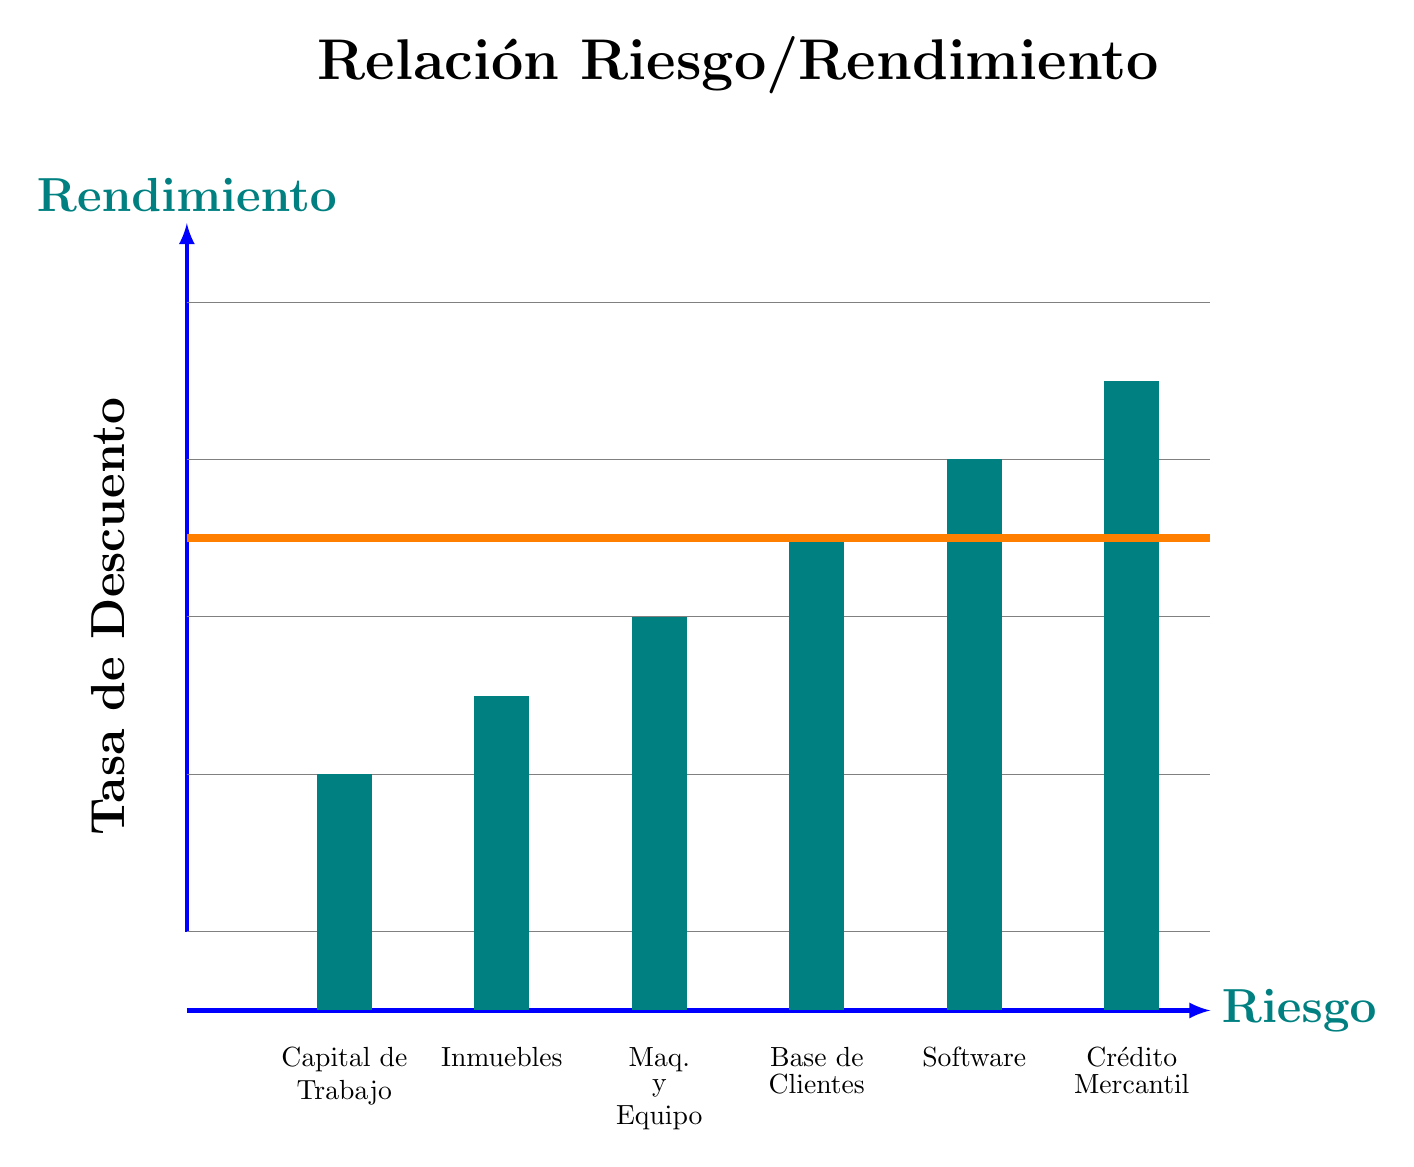
\begin{tikzpicture}[>=latex, scale=2]
	\draw [ultra thick,->,blue] (0,0) -- (6.5,0)
	node [right] {\LARGE \color{teal} \textbf{Riesgo}};
	\draw [ultra thick,->,blue] (0,0.5) -- (0,5)
	node [above] {\LARGE \color{teal} \textbf{Rendimiento}};
	\foreach \n in {1,...,5} \draw [help lines] (0,\n-0.5) --++ (6.5,0);
	\foreach \n/\text in {
		1/ \shortstack{Capital de \\ Trabajo},
		2/Inmuebles,
		3/ \shortstack{Maq. \\ y \\ Equipo},
		4/ \shortstack{Base de \\ Clientes},
		5/ Software,
		6/ \shortstack{Crédito \\ Mercantil}
	} 
	\draw [line width=7mm, teal] 
	(\n,0) node [below] {\color{black} \text} --++ (0,1+\n/2);
	\draw [line width=1mm,orange] (0,3) -- (6.5,3);
	\node  at (-0.5,2.5) {\rotatebox{90}{\LARGE \textbf{Tasa de Descuento}}};
	\node at (3.5,6) {\huge \textbf{Relación Riesgo/Rendimiento}};
\end{tikzpicture}

\end{document}
